\documentclass[a4paper,12pt]{article}
\RequirePackage[l2tabu, orthodox]{nag}
\usepackage{setspace}
\usepackage{amsfonts}
\usepackage{amsmath}
\usepackage{graphicx}
%Enable fr support
\usepackage[utf8]{inputenc} 
\usepackage[T1]{fontenc} 
\usepackage{lmodern} % load a font with all the characters

%Assign document variables
\date{\today}
\title{Projet Final;}
\author{tmp}
\newcommand{\Author}{Kevin Belisle}
\newcommand{\Authorr}{Michael Leblanc}
\newcommand{\Authorrr}{Temp}
\newcommand{\Teacher}{Michel Boyer}
\newcommand{\ClassNum}{IFT-2935}
\newcommand{\ClassName}{Bases de données}
\newcommand{\DateMMMMYYYY}{Mai 2018}
\newcommand{\tab}[1]{\hspace{.05\textwidth}\rlap{#1}}
\makeatletter
%Custom Header & Footer
\usepackage{fancyhdr}
\pagestyle{fancy}
\fancyhf{}
\fancyhead[L]{\@title}
\fancyhead[R]{\thepage}
\fancyfoot[L]{Kevin Belisle \& Michael Leblanc \& Temp}
\fancyfoot[R]{\DateMMMMYYYY}
\renewcommand{\footrulewidth}{0.4pt}% default is 0pt

\begin{document}
	\begin{titlepage} 
		\begin{center}
			\textsc{\normalsize Université de Montréal}\\[2.25cm]
			 
			\textsc{\LARGE \@title}\\[2.25cm]
			
			\textsc{\small Par}\\[0.25cm]
			\textsc{\LARGE \Author}\\[0.25cm]
			\textsc{\normalsize (20018469)}\\[0.25cm]
			\textsc{\LARGE \Authorr}\\[0.25cm]
			\textsc{\normalsize (20005779)}\\[0.25cm]
			\textsc{\LARGE \Authorrr}\\[0.25cm]
			\textsc{\normalsize (00000000)}\\[2cm]
			
			\textsc{\normalsize Baccalauréat en informatique}\\
			\textsc{\normalsize Faculté des arts et des sciences}\\[2.25cm]
			
			\textsc{\small Travail présenté à \Teacher}\\
			\textsc{\small Dans le cadre du cours \ClassNum}\\
			\textsc{\small \ClassName}\\[2.25cm]
			
			\textsc{\normalsize \DateMMMMYYYY}\\[1.5cm]
		\end{center}
	\end{titlepage}
	\begin{spacing}{1}
	%La représentation E-A de la base relationnelle accompagné d'explications%
	\section*{Modèle entité-association}
	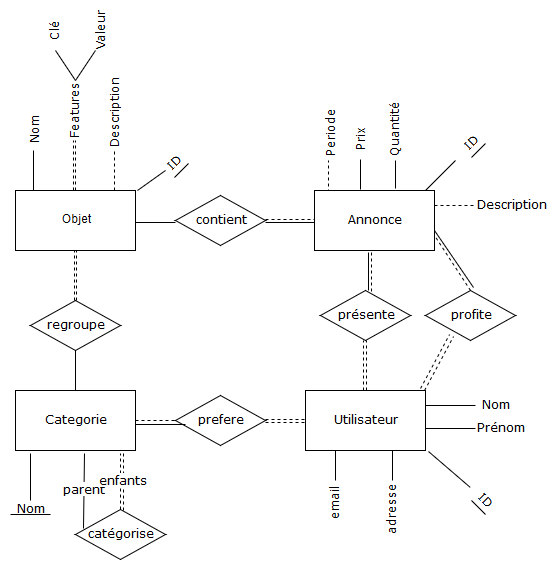
\includegraphics[scale=0.6]{modeleEA.png}
	\subsection*{Catégorie}
	TODO
	\subsection*{Objet}
	TODO
	\subsection*{Annonce}
	TODO
	\subsection*{Utilisateur}
	TODO
	%Le schéma relationnel de la base%
	\section*{Schéma relationnel}
	Utilisateur(\underline{iduser}, prenom, nom, email, adresse)\\
	Categorie(\underline{ncat},\#pcat)\\
	Prefere(\underline{\#iduser},\underline{\#ncat})\\
	Objet(\underline{idobj}, name, ncat, odesc)\\
	Feature(\underline{\#idobj},\underline{fname},fvalue)\\
	Annonce(\underline{idannonce},\#idobj,\#idvendeur,datedebut,datefin,prix,qte,description)\\
	Partage(\underline{\#idacheteur},\underline{\#idannonce},\underline{data})
	% PK %
	% Formats standard %
	% Separe ou duplication %
	% Choix d'implementation %
	\section*{Explication du DDL}
	\subsection*{Catégorie}
	Nous avons choisi le nom de la catégorie (ncat) comme clé primaire puisque c'est le seul et unique champ propre à la table. Le champs pcat réfère à la catégorie parent (NULL si aucun parent) ainsi il est possible de trouver tous les objets faisant partie de la catégorie choisie et de ces enfants.
	\subsection*{Objet}
	TODO
	\subsection*{Annonce}
	TODO
	\subsection*{Utilisateur}
	TODO
	% L'ensemble des requêtes en SQL et explication du résultat attendu %
	\section*{Requêtes SQL}
	\subsection*{Vues}
	TODO
	\subsection*{SELECT}
	TODO
	\subsection*{DML}
	TODO
	% Captures d’écran de l’application avec description de fonctionnement de l’application%
	\section*{Guide Utilisateur}
	TODO
	\end{spacing}                                                 
\end{document} 